\documentclass[sigconf]{acmart}
\usepackage{arydshln}

\usepackage{booktabs} % For formal tables


% Copyright
%\setcopyright{none}
%\setcopyright{acmcopyright}
%\setcopyright{acmlicensed}
\setcopyright{rightsretained}
%\setcopyright{usgov}
%\setcopyright{usgovmixed}
%\setcopyright{cagov}
%\setcopyright{cagovmixed}


% DOI
\acmDOI{10.475/123_4}

% ISBN
\acmISBN{123-4567-24-567/08/06}

%Conference
\acmConference[WOODSTOCK'97]{ACM Woodstock conference}{July 1997}{El
  Paso, Texas USA} 
\acmYear{1997}
\copyrightyear{2016}


\acmArticle{4}
\acmPrice{15.00}

% These commands are optional
%\acmBooktitle{Transactions of the ACM Woodstock conference}
%\editor{Jennifer B. Sartor}
%\editor{Theo D'Hondt}
%\editor{Wolfgang De Meuter}


\begin{document}
\title{Towards Dynamic Load Balancing Policies in Software-Defined Storage}
%\titlenote{Produces the permission block, and
%  copyright information}
%\subtitle{Extended Abstract}
%\subtitlenote{The full version of the author's guide is available as
%  \texttt{acmart.pdf} document}


\author{Michael A. Sevilla}
\authornote{Work done while interning at LANL.}
\affiliation{%
  \institution{University of California, Santa Cruz}
}
\email{msevilla@soe.ucsc.edu}

\author{Brad Settlemyer}
\affiliation{%
  \institution{Los Alamos National Lab}
}
\email{bws@lanl.gov}

\author{Carlos Maltzahn}
\affiliation{%
  \institution{University of California, Santa Cruz}
}
\email{carlosm@soe.ucsc.edu}

\begin{abstract}
Lorem ipsum dolor sit amet, consectetur adipiscing elit. Sed enim libero,
vestibulum quis efficitur et, commodo vitae lorem. Proin metus odio, molestie
sit amet magna at, eleifend lobortis neque. Mauris placerat arcu ac lacus
venenatis auctor. Aliquam rutrum non tellus vitae tempor. Aliquam erat
volutpat. Duis enim leo, condimentum tincidunt posuere nec, ultricies vitae
nisi. Aliquam efficitur massa felis, in tempus ante pretium ac. Cras eget
luctus felis, id eleifend nulla.
\end{abstract}

%
% The code below should be generated by the tool at
% http://dl.acm.org/ccs.cfm
% Please copy and paste the code instead of the example below. 
%
%\begin{CCSXML}
%<ccs2012>
% <concept>
%  <concept_id>10010520.10010553.10010562</concept_id>
%  <concept_desc>Computer systems organization~Embedded systems</concept_desc>
%  <concept_significance>500</concept_significance>
% </concept>
% <concept>
%  <concept_id>10010520.10010575.10010755</concept_id>
%  <concept_desc>Computer systems organization~Redundancy</concept_desc>
%  <concept_significance>300</concept_significance>
% </concept>
% <concept>
%  <concept_id>10010520.10010553.10010554</concept_id>
%  <concept_desc>Computer systems organization~Robotics</concept_desc>
%  <concept_significance>100</concept_significance>
% </concept>
% <concept>
%  <concept_id>10003033.10003083.10003095</concept_id>
%  <concept_desc>Networks~Network reliability</concept_desc>
%  <concept_significance>100</concept_significance>
% </concept>
%</ccs2012>  
%\end{CCSXML}

%\ccsdesc[500]{Computer systems organization~Embedded systems}
%\ccsdesc[300]{Computer systems organization~Redundancy}
%\ccsdesc{Computer systems organization~Robotics}
%\ccsdesc[100]{Networks~Network reliability}
%
%
%\keywords{ACM proceedings, \LaTeX, text tagging}


\maketitle

\section{Introduction}

\begin{itemize}
  \item key-value stores
  \begin{enumerate}
    \item Fine scale annotation
    \item Scalability
    \item flexible, extensible formats
  \end{enumerate}
  \item science
  \begin{enumerate}
    \item entropy is increasing
    \item graph showing regimes (key distribution, popularity over time)
  \end{enumerate}
\end{itemize}

Hypothesis: re-distributing keys requires dynamic load balancing policies\cite{perez:jctc20150parsplice}



%% What is the problem?
%Load balancing is a useful tool for optimizing performance in systems that
%service highly accessed data\footnote{In this paper, we use the term ``data" to
%refer to the partitioned key-value pairs AND file system metadata.} but
%deciding how to make the migrations is a risky trade-off. In this paper, we
%show that a one-size-fits-all data load balancing policy is not sufficient for
%even the simplest of HPC applications and argue for a dynamic load balancing
%policy.
%
%% Explain techniques
%Resource migration is the key mechanism for load balancing. In storage, data
%can be distributed to alleviate overloaded servers or it can be concentrated to
%exploit locality. These techniques are at odds and selecting the wrong
%technique can have catastrophic consequences. For example, migrating data to an
%already overloaded server or increasing the network hops by spreading data
%across an underutilized cluster will impact performance negatively.
%
%% Why is concentration vs. distribution difficult?
%Unfortunately, deciding which optimization to use is difficult to reason about,
%especially with the scale and complexity of today's HPC architectures. While
%the mechanisms are usually built into the systems, the policies often times
%less refined and much more sensitive to the workload. So a system may have the
%ability exploit locality using techniques like bulk operations, multiple
%partition strategies, secondary indexes, and caching but deciding when, where,
%and how to use them is workload dependent and difficult to figure out.
%
%% What we did in the paper
%This paper takes an API designed to migrate file system metadata and applies it
%to an HPC key-value store.  The API helps control distribution and
%concentration by letting the administrator define how to migrate load, where to
%migrate load, and how much load to migrate. While designed for a different
%domains, this API encompasses many of the same properties we need for an HPC
%key-value store, namely:
%
%\begin{itemize}
%  \item services small/frequent requests
%  \item popularity drives distribution
%  \item locality drives concentration
%\end{itemize}
%
%\begin{figure}[t]
%  \noindent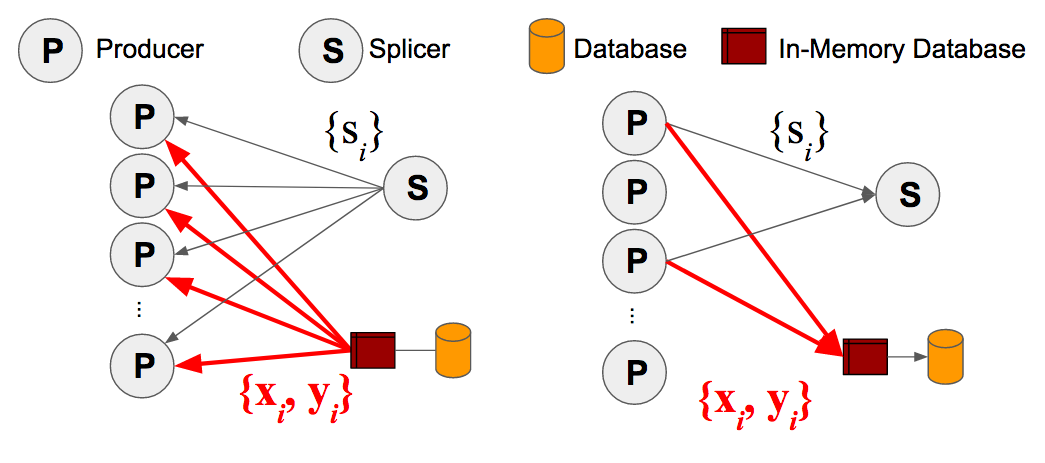
\includegraphics[width=19pc,angle=0]{figures/arch-parsplice.png}\\
%  \caption{ParSplice is a ready-heavy HPC application where producers use a
%  database for consistency. Replacing the single-node database with HXHIM
%  improves performance with load balancing.
%  \label{fig:arch-parsplice}}
%\end{figure}
%
%% Why is HXHIM a good fit?
%To show the efficacy of this approach, we examine the ParSplice molecular
%dynamics simulation application shown in Figure~\ref{fig:arch-parsplice}.
%ParSplice uses a single-node database for consistency, where producers, \(P\),
%push and pull coordinates, \{\(x_i, y_i\)\}, based on the segments,
%\{\(s_i\)\}, assigned by the splicer, \(S\). In this paper, we replace the
%database with a distributed key-value store designed for HPC enjoy performance
%optimizations for:
%
%\begin{itemize}
%  \item \texttt{put()} because of the distributed sync and load balancing based on:
%  \begin{itemize}
%    \item lazy synchronization with tombstones and RPCs
%    \item strong synchronization with consensus and blocking
%  \end{itemize}
%  \item \texttt{get()} because of the load balancing
%\end{itemize}
%
%It has 4 phases:
%
%\begin{enumerate}
%
%  \item splicer (S) tells producers (P) to compute segments for state \(s_i\)
%
%  \item P's pull initial coordinates \{\(x_i, y_i\)\} from database
%
%  \item a P inserts completed coordinates for segment \(s_i\) into database and
%  S broadcasts next segment(s) \(s_j\) 
%
%  \item P's pull new segment coordinates \{\(x_j, y_j\)\}
%\end{enumerate}
%
%, which has both a high computational footprint and data locality.
%The former suggests distribution to avoid hot spots while the latter encourages
%concentration to leverage the database's secondary indeices, bulk operations,
%and key redistribution functionality. 
%
%% Why is HXHIM a good fit?
%To show this approach at scale we study
%ParSplice~\cite{perez:jctc20150parsplice}, an HPC dynamics simulator that has
%both a high computation footprint, which suggests distribution to avoid hot
%spots, and data locality, which alternatively encourages concentration so the
%key-value store can use its functionality for secondary indices, bulk
%operations, and key redistribution. ParSplice uses both molecular dynamic (MD)
%and accelerated molecular dynamic methods (AMD) for simulations with long
%periods of inactivity and short periods of ``interesting" events.  Molecules in
%periods with many events are simulated with MD methods, which are exact but can
%only be run for a fixed, short period of time because the cumulative error
%grows so large. Alternatively, longer trajectories are simulated with AMD
%methods, which use statistics and parallelization to show the less precise
%state-to-tate trajectories. ParSplice tackles ``low-barrier problems", where
%the types of energy barriers separating states of the system are non-uniform
%(i.e. some require less energy than others). It chops long trajectories into
%parallelizable units called segments, where the segments can also be spliced
%together to form longer trajectories; this approach allows ParSplice to trade
%off accuracy for speed in a configurable way.
%
%% How is ParSplice implemented?
%ParSplice stores segments in a database while it runs. The splicer pastes
%segments generated by \(n\) producers.
%
%% What do we contribute?
%In this paper, we make the following contributions:
%
%\begin{enumerate}
%
%  \item protype that controls concentration and distribution using the bulk
%  operations, secondary indicies, and cursor types mechanisms
%  from~\cite{greenberg:hotstorage2015-mdhim}. 
%
%  \item quantifies benefits of server/client-side caching, many small messages,
%  and bulk operations.
%
%\end{enumerate}

\section{Background}

\subsection{ParSplice}
\label{sec:parsplice}

\begin{figure}[t]
  \noindent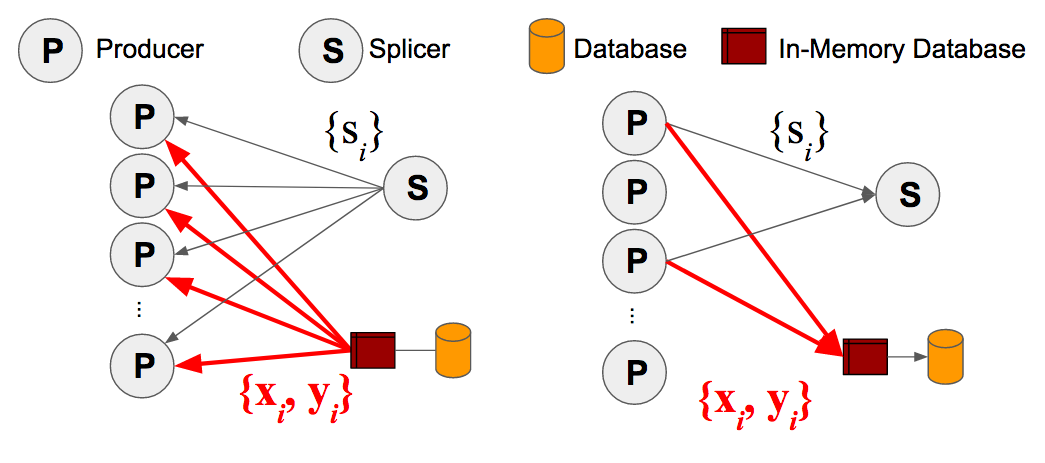
\includegraphics[width=19pc,angle=0]{figures/arch-parsplice.png}\\
  \caption{ParSplice is a ready-heavy HPC application where producers use a
  database for consistency. Replacing the single-node database with HXHIM
  improves performance with load balancing.
  \label{fig:arch-parsplice}}
\end{figure}


ParSplice~\cite{perez:jctc20150parsplice} is a molecular dynamics simulation
developed at LANL. It has 4 phases, as depicted in Figure~\ref{fig:arch-parsplice}:

\begin{enumerate}

  \item splicer (S) tells producers (P) to compute segments for state \(s_i\)

  \item P`s pull initial coordinates \{\(x_i, y_i\)\} from database

  \item a P inserts completed coordinates for segment \(s_i\) into database and
  S broadcasts next segment(s) \(s_j\) 

  \item P`s pull new segment coordinates \{\(x_j, y_j\)\}

\end{enumerate}

The database is single node (LevelDB or BerkeleyDB) with caches in front. Our
goal is to replace this architecture with a distributed key-value store to
solve the immediate sync problems that the ParSplice team is facting. Sliding
in something like MDHIM~\cite{greenberg:hotstorage2015-mdhim} has the added
benefit of enabling load balancing. ParSplice has distinct workload phases and
a well-known keyspace (Figure~\ref{fig:methodology-keyspace}) so its
performance should improve with better load balancing.

\subsection{MDHIM: Key-Value Store for HPC}
\label{sec:hxhim}

\begin{figure}[tb]
  \noindent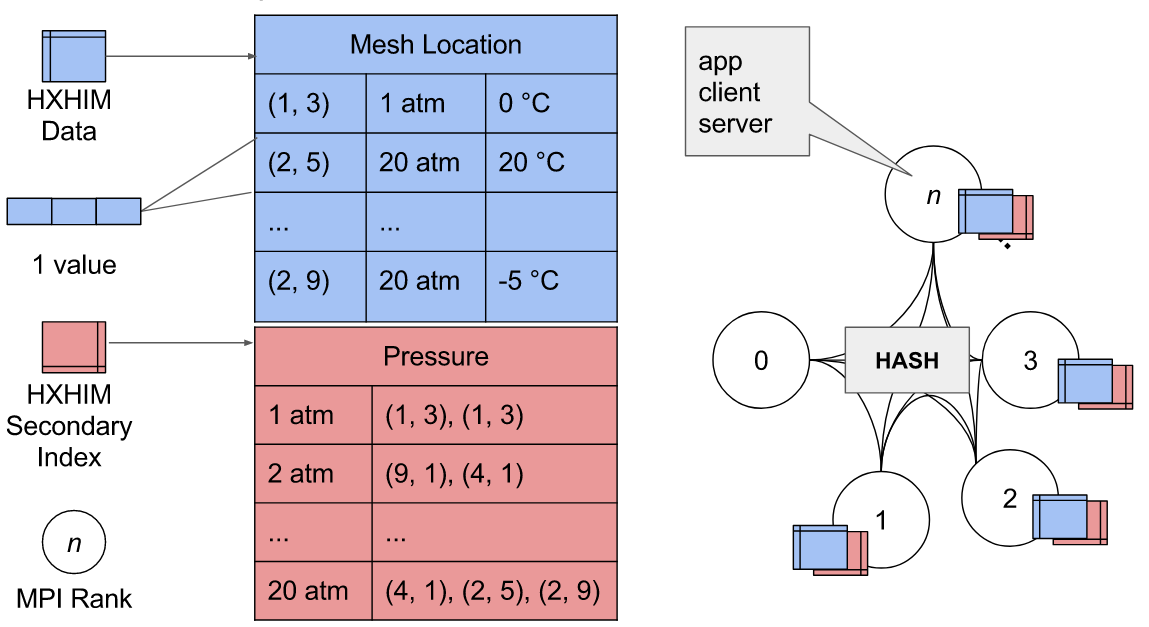
\includegraphics[width=19pc,angle=0]{figures/arch-hxhim.png}\\
  \caption{The MDHIM architecture.}
  \label{fig:arch-hxhim}
\end{figure}

% What is MDHIM
MDHIM is a key-value store designed for HPC architectures and multi-dimensional
data. It is based off MDHIM~\cite{greenberg:hotstorage2015-mdhim}, the
multi-dimensional indexing middleware. Figure~\ref{fig:arch-hxhim} has a crude
sketch of the MDHIM architecture. Each MPI rank has an instance of the
application, which has the client library linked in. An MPI rank can also have
a ``range server", which stores the key-value pairs in a local databse (either
LevelDB or MySQL). Data is located with a consistent hash, which is
configurable.

% What are the indexes?
The primary and secondary indices shown on the right side of
Figure~\ref{fig:arch-hxhim} are views of the data that the range server
manages.  The primary index is the same hash used by the global partitioner.
The secondary index or indices are user-defined tables organized in a different
way from the primary index. The goal of the secondary indices is to speed up
queries that need to aggregate dat ({\it e.g.} find the maximum values). In the
example, the range server and the key in the primary index is located with a
hash of the mesh location. The secondary index is organized by pressure, so
queries asking for a certain atmosphere can be serviced in O\(1\), consisting
of one lookup in the pressure index and one lookup into the primary index.

% Why is it tailored to HPC?
MDHIM tailors its mechanisms and policies to HPC, showing improved performance
over cloud-based key-value stores like Cassandra. It has cursor types for
walking the key-value store, bulk operations for exploiting data locality,
per-job server spawning, and pluggable backends for its local database and
network type (infiniband/RDMA). Its policies are flexible, supporting
customized partitioning strategies and user-defined secondary indices. This
allows the system to choose whether to send load to the client or server.

%\subsection{Comparing Mantle and MDHIM}
%\begin{table*}
%\centering
%\begin{tabular}[tb]{ r | l | l | l | l }
%                       & 
%                       & \multicolumn{1}{c|}{\centering Both} 
%                       & \multicolumn{1}{c|}{\centering Mantle/CephFS}
%                       & \multicolumn{1}{c}{\centering MDHIM}
%                       \\\hline
%  workload   & characteristics     & small/frequent requests  & data access            & data management \\
%             & write-intensive     & partition across cluster & fragment directories*  & NOT IMPLEMENTED \\
%             & read-intensive      & replicate across cluster & copy directories*      & NOT IMPLEMENTED \\\hdashline
%  system     & measure workload    & yes                      & directory temperature  & range server counts \\
%  mechanisms & measure utilization & yes                      & CPU, network, memory   & range server buffer size \\
%             & migrate resources   & almost                   & \texttt{export\_dir()} & \texttt{mdhimB}\{\texttt{Get}, \texttt{Put}\}\texttt{()} \\
%             & partition resources & yes                      & subtrees \& dirfrags   & secondary index, cursor type, bulk operations\\\hdashline
%  migration  & interval            & configurable             & every 10 seconds       & every query \\
%  decisions  & global state        & decentralized decisions  & heartbeats for metrics & NOT IMPLEMENTED \\
%  \multicolumn{5}{c}{}\\
%  \multicolumn{5}{c}{\tiny *Mechanisms implemented in CephFS, not integrated into Mantle}
%\end{tabular}
%\caption{Comparing the design goals and implementatons of Mantle and MDHIM.}
%\label{fig:arch-comparison}
%\end{table*}
%
%% Why are the designed for the same type of workload?
%The ``Both" column of Table~\ref{fig:arch-comparison} shows how Mantle and
%MDHIM have similar designs. The workloads are very similar as the the services
%respond to small and frequent requests, which results in hot spots and flash
%crowds. As a result, popularity of the data, not the size, drives distribution
%in both systems. Both workloads also have data locality so the systems have
%mechanisms for leveraging requests with similar semantic meaning.  Finally, the
%overall design of both systems is decentralized meaning that there is no
%centralized scheduler and each server has an inconsistent global view.
%
%% What are the challenges?
%Despite the similarities, integrating the Mantle API with MDHIM has both design
%and technical challenges. Mantle is reactive to the workload as opposed to
%MDHIM migrations, which are triggered based on the request type. As a result,
%Mantle has functionality for exchanging server utilization (CPU, network,
%memory) and workload (tracks request types). MDHIM 
%
%
%%This paper takes the API and load balancers designed in
%%Mantle~\cite{sevilla:sc15-mantle}, the programmabile file system metadata load
%%balancer for Ceph, and applies them to
%%MDHIM~\cite{greenberg:hotstorage2015-mdhim}, the distributed key-value store
%%designed for HPC.
%
%
%
%Results should show, In order from most likely to least likely:
%
%\begin{enumerate}
%
%  \item HPC key-value store workloads are structured (because they are mostly
%  workflows and simulations) that their job phases can be learned and exploited
%  using dynamic load balancing policies.
%
%  \item HPC key-value store workloads are so structured that one
%  policy-fits-all
%
%  \item HPC key-value store workloads are not structured enough to be learned
%
%  \item HPC key-value store workload hotspots/flash crowds are too fast to be
%  exploited
%
%\end{enumerate}

\section{Methodology: Extracting Mantle Library}

\begin{itemize}
  \item C bindings for Mantle
\end{itemize}

\subsection{Pluggable Interfaces}

\begin{figure}[tb]
  \noindent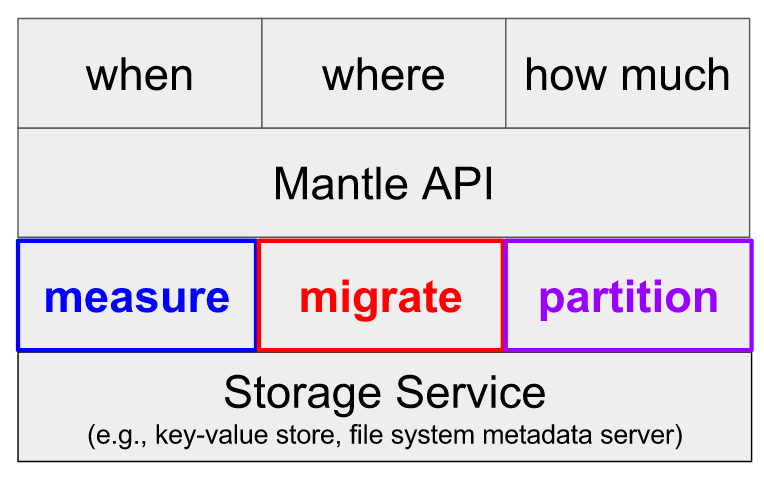
\includegraphics[width=19pc,angle=0]{figures/mantle-pluggable-interfaces.png}\\
  \caption{The storage service must: \textcolor{blue}{\textbf{measure}}
  resource usage, \textcolor{red}{\textbf{migrate}} resources, and
  \textcolor{purple}{\textbf{partition}} resources. }
  \label{fig:mantle-pluggable-interfaces}
\end{figure}

\subsubsection{Measure}

The metrics measured should help the system decide ``when" to migrate server
load. They should:

\begin{itemize}
  \item tell us about the state of the server or cluster
  \item provide some value of load, so we can partition/send it
\end{itemize}

In Ceph: global and local metrics ({\it e.g.}, CPU utilization, file system operation counts) \\

In HXHIM: ???\\

\subsubsection{Migrate}

In Ceph: \texttt{export\_dir()}

In HXHIM: \texttt{mdhimBPut()}, \texttt{mdhimBGet()}, ``adjusting ... keys" ???

\subsubsection{Partition}

In Ceph: subtrees and directory fragments

In HXHIM: secondary indices, cursor types, bul operations

\section{Results}
\label{sec:results}

%IT HAS 8K keys!  How did we take these measurements
\subsection{ParSplice Keyspace Analysis}
\label{sec:parsplice-keyspace-analysis}

We examine the keyspace size and access patterns using
Figures~\ref{fig:futurework-regimes} and~\ref{fig:methodology-keyspace}. These
results are collected using the performance and keyspace counters described in
Section~\S\ref{sec:parsplice-instrumentation}.

\subsubsection*{An active but small keyspace} The black text annotations in
Figure~\ref{fig:methodology-keyspace} show that the keyspace size ranges from
about 10K keys for 32 workers to 100K keys for 1048 workers.  The bars show
\(50-100\times\) as many reads (\texttt{get()}) as writes (\texttt{put()}).
Workers read the same key for extended periods because the trajectory segment
is stuck in a superbasin composed of local minima, so many coordinates are
needed before the trajectory moves on. Writes only occur for the final state of
segments generated by workers; their magnitude is smaller than reads because
the caches ignore redundant put requests. The number of read and write requests
are highest at the beginning of the run when workers generate segements for the
same state, which is cheap. This type of keyspace encourages replication across
a cluster.  

\subsubsection*{Entropy increases over time} The reads per second in
Figure~\ref{fig:futurework-regimes} show that the number of requests decreases
and the number of active keys increases over time. The resulting imbalance for
the two growth rates in Figure~\ref{fig:futurework-regimes} are shown in
Figure~\ref{fig:methodology-keys}, where reads are plotted for each unique
state (\(x\) axis). Keys are more popular than others (up to \(5\times\))
because workers start generating states with different coordinates later in the
run.

\subsubsection*{Entropy growth is structured} The access patterns reflect the
locality of computation: workers stuck in state basins generate segments with
similar coordinates. The growth rate, temperature, and number of workers
changes that locality, which has an effect on the structure of the keyspace.
Figure~\ref{fig:methodology-keys} shows that the number of reads changes with
different growth rates, but that spatial locality is similiar ({\it e.g.}, some
keys are stil \(5\times\) more popular than others).
Figure~\ref{fig:futurework-regimes} shows how entropy for different growth
rates has temporal locality, as the reads per second for 1M looks like the
reads per second for 100K stretched out along the time axis.  Trends also exist
for temperature and number of workers but are ommitted here for space. This
structure means that we can learn the regimes and adapt the storage system to
it. 

\begin{figure}[tbh]
  \noindent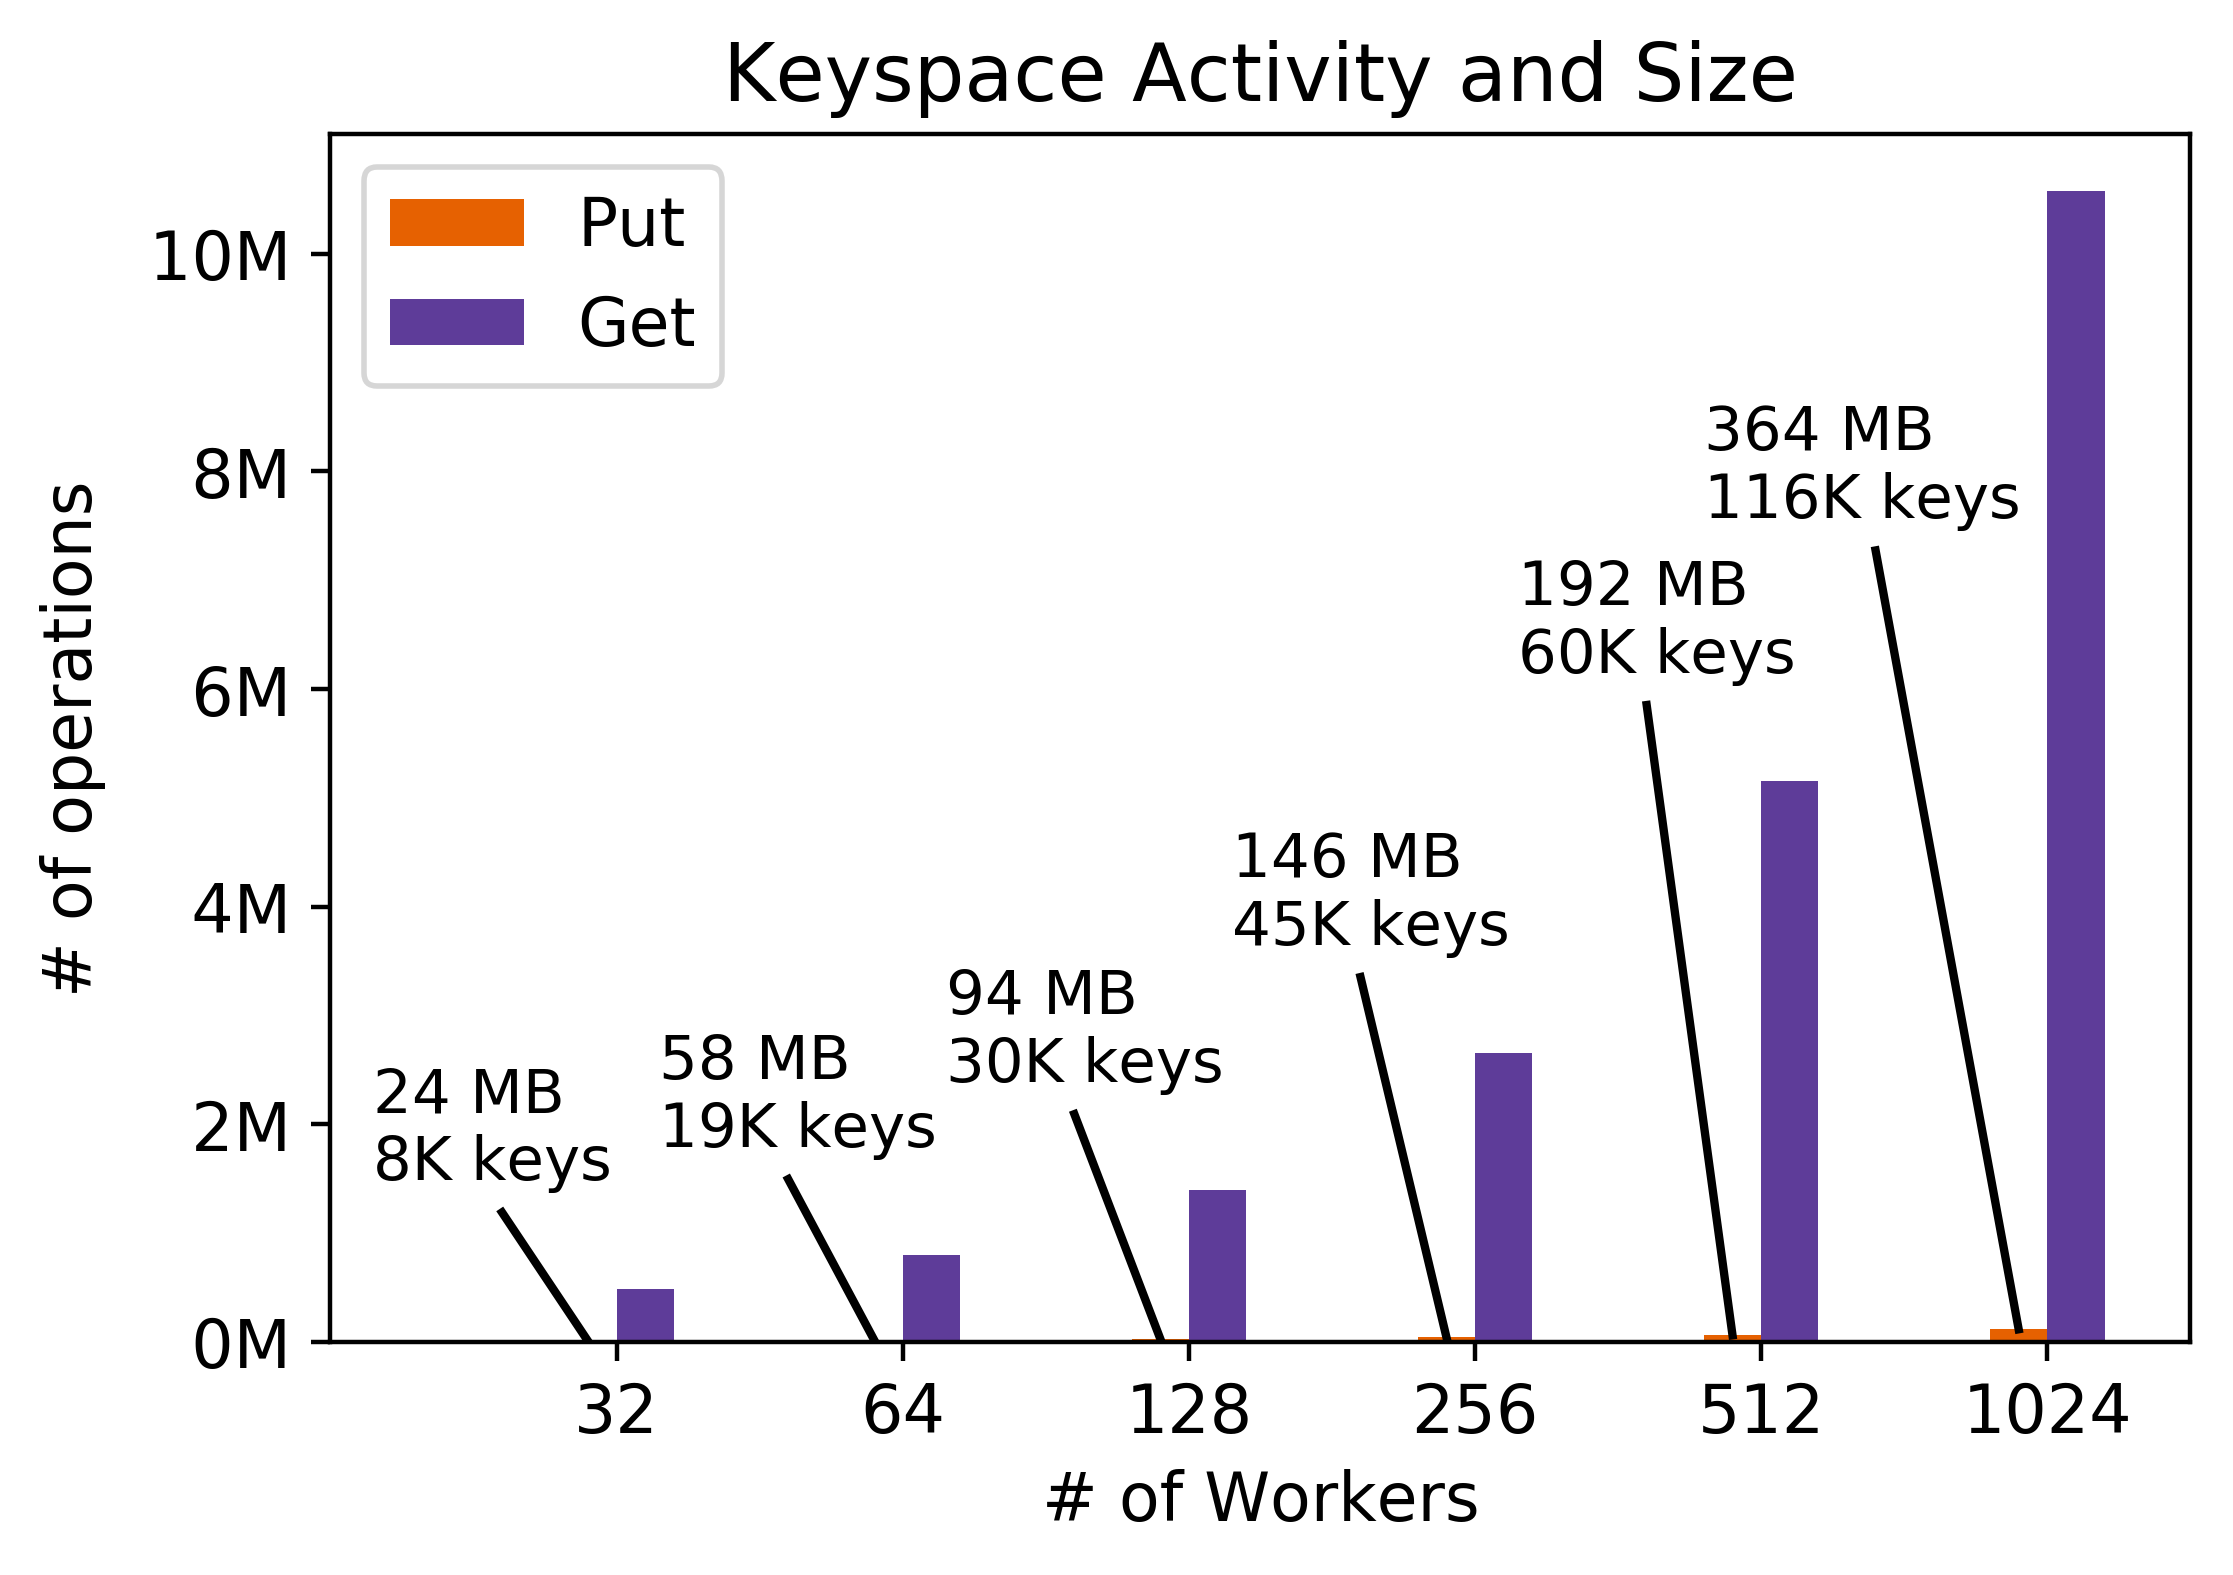
\includegraphics[width=0.45\textwidth]{figures/methodology-keyspace.png}\\
  \caption{The keyspace size is small (numbers above bars) but must
  satisfy many reads as workers calculate new segments. The active keyspace is
  difficult to predict a priori but the optimal load balancing strategy strikes a
  good balance between preformance and utilization. 
  \label{fig:methodology-keyspace}}
\end{figure}

\begin{figure}[tbh]
  \noindent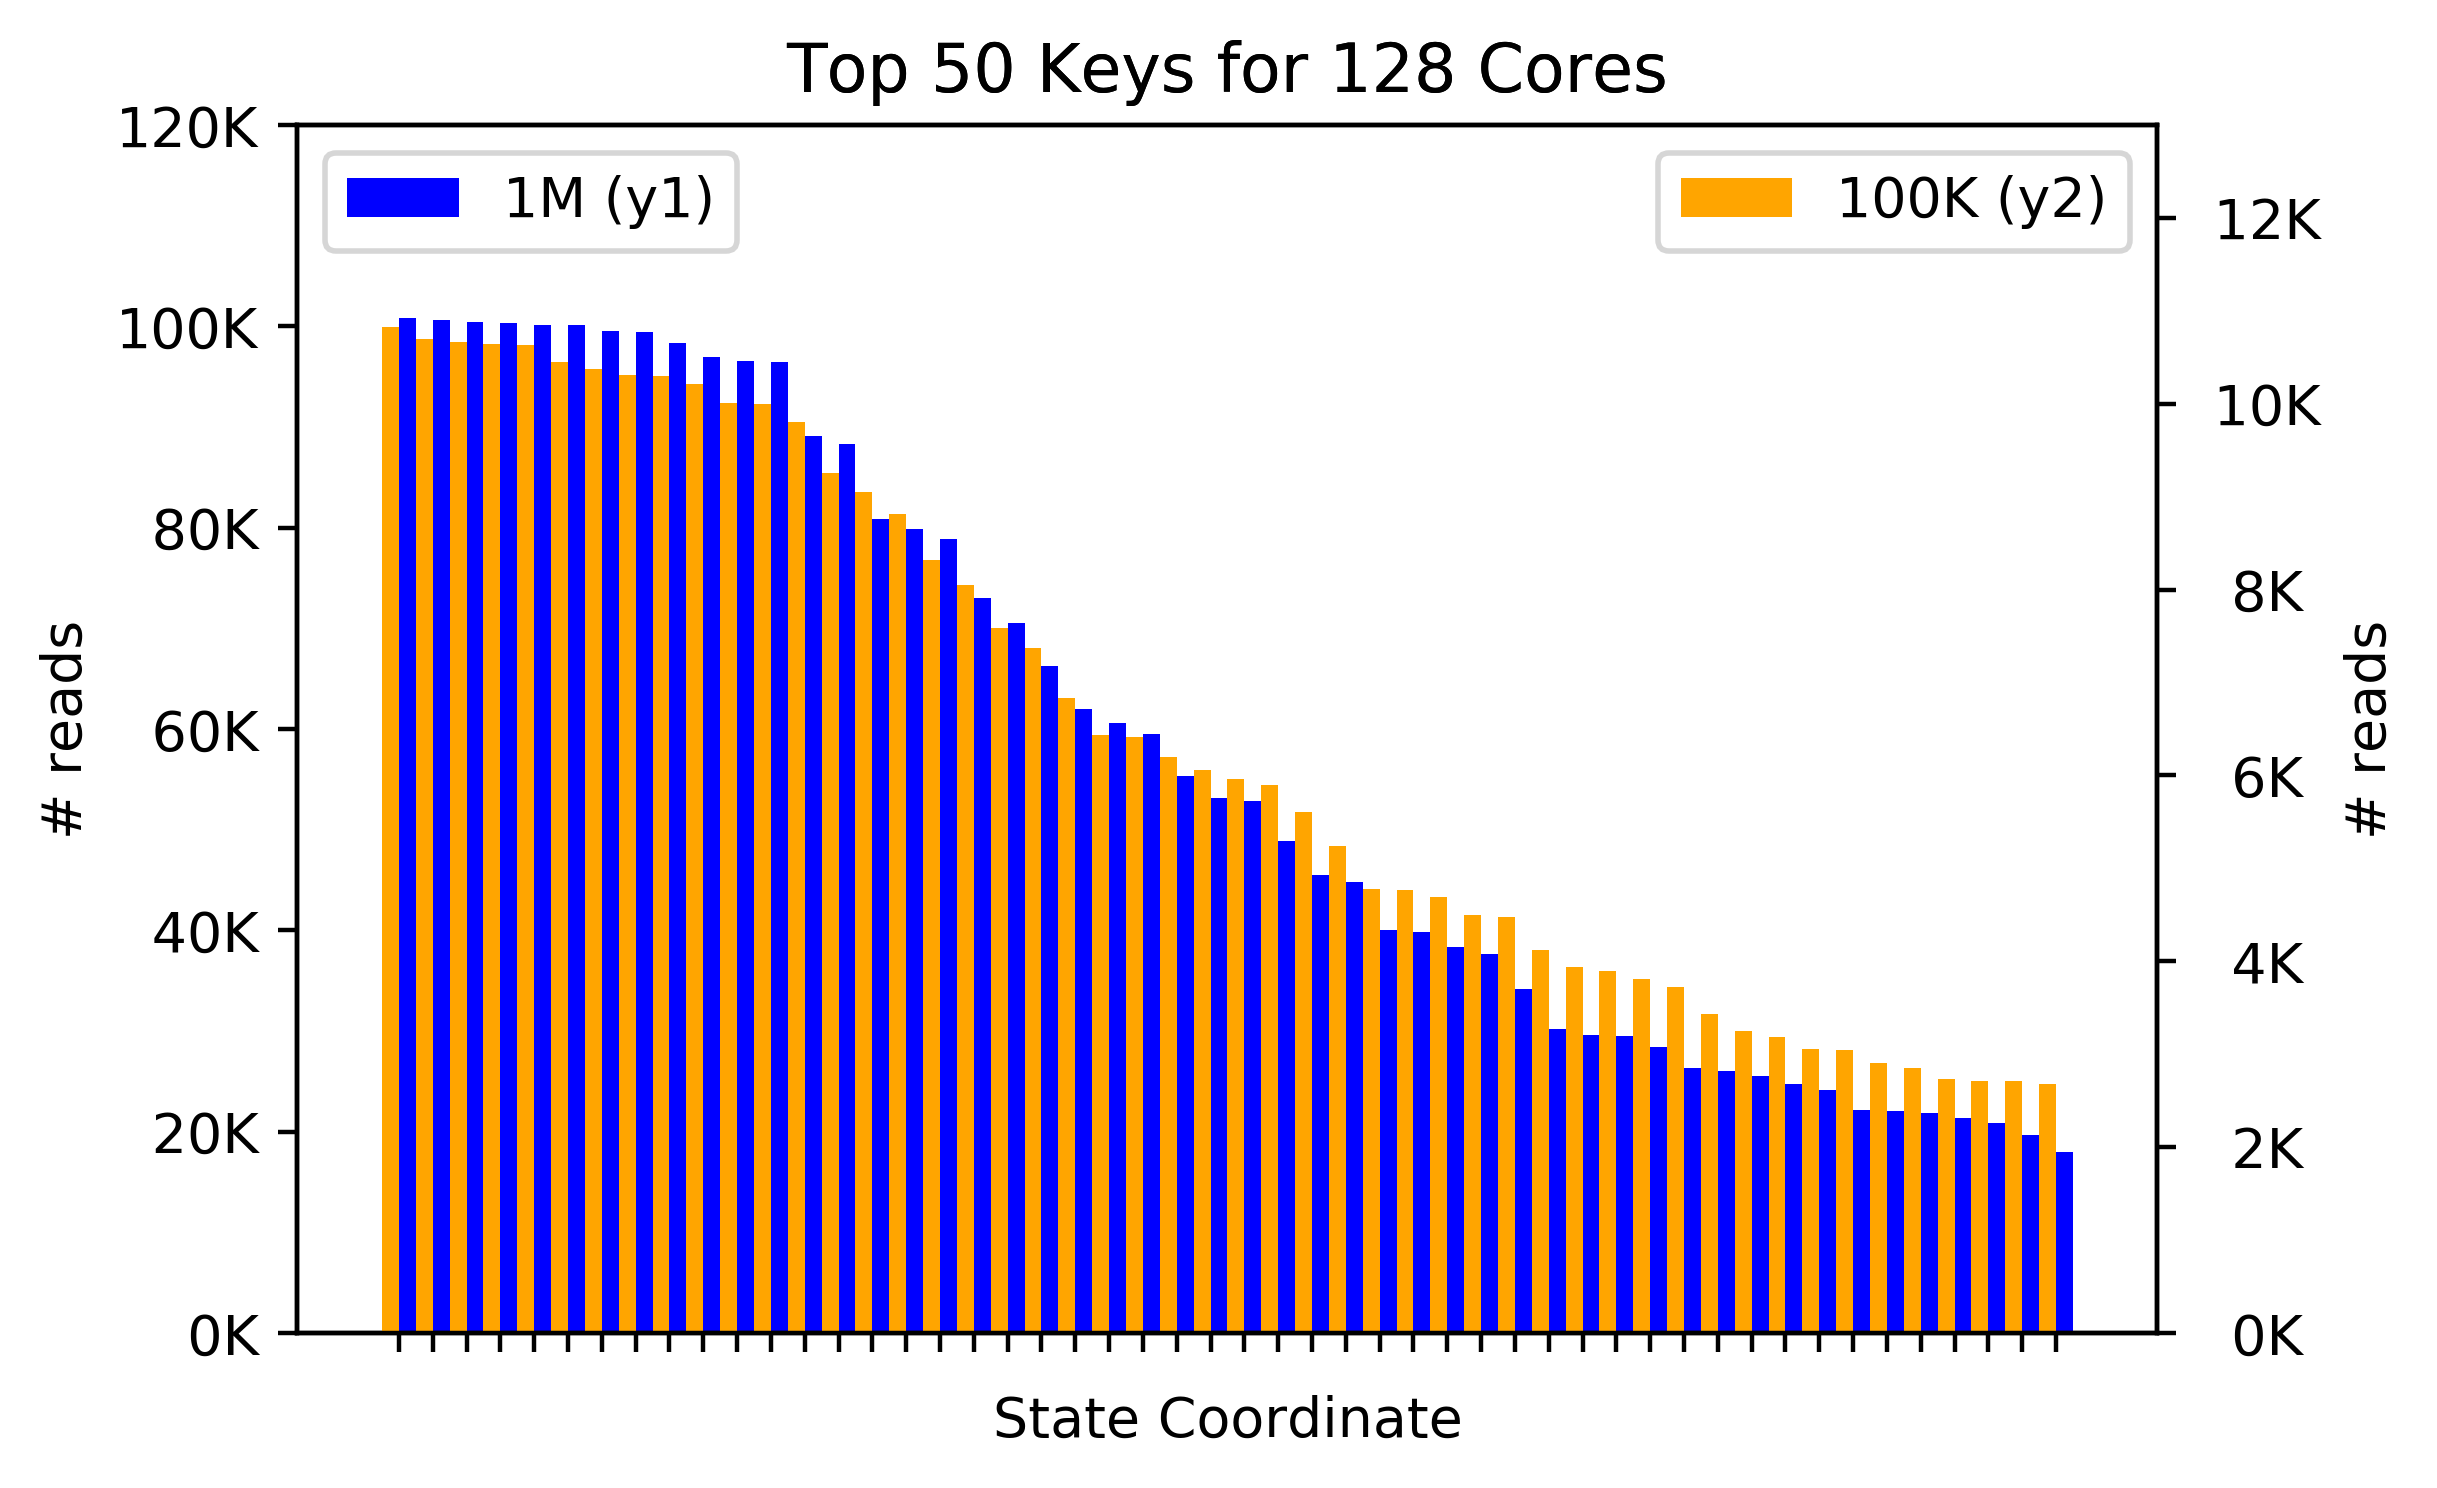
\includegraphics[width=0.45\textwidth]{figures/methodology-keys.png}\\
  \caption{The keyspace imbalance is due to workers generating deep
  trajectories and reading the same coordinates. Over time, the accesses get
  dispersed across different coordinates resulting in some keys being more
  popular than others.\label{fig:methodology-keys}}
\end{figure}

\subsection{Positive Effects of Load Balancing}
\label{sec:positive-effects-of-load-balancing}

% results: cache size trade-offs
The results for different cache sizes, described in
Section~\S\ref{sec:static-load-balancing}, for a growth rate of 100K over a 2.5
hour run is shown in the left two plots of
Figure~\ref{fig:methodology-tradeoff}.  ``Baseline" is the performance of
unmodified ParSplice  measured in trajectory duration (\(y\)-axis) and
utilization is measured with memory footprint (\(y2\) axis) of just the cache.
``Static Load Balancing Policies" shares the \(y\)-axis and shows the trade-off
for different cache sizes. The error bars are the standard deviation of 3 runs. 

% results: raw numbers
Although the keyspace grows to 150K, a 100K key cache achieves 99\% of the
peformance. Decreasing the cache degrades performance and predictability.  Not
suprisingly, the memory usage all decreases with the cache size and although we
only save 0.4GB, larger and more complicated runs use up to 4GB, which is 3\%
of the 128GB on each node.  While this result is not unexpected, it nonetheless
achieves our goal of showing the benefits of load balancing keys across nodes
and that smaller caches on each node are an effective way to save memory
without completely sacrificing performance.

\begin{figure*}[tbh]
  \noindent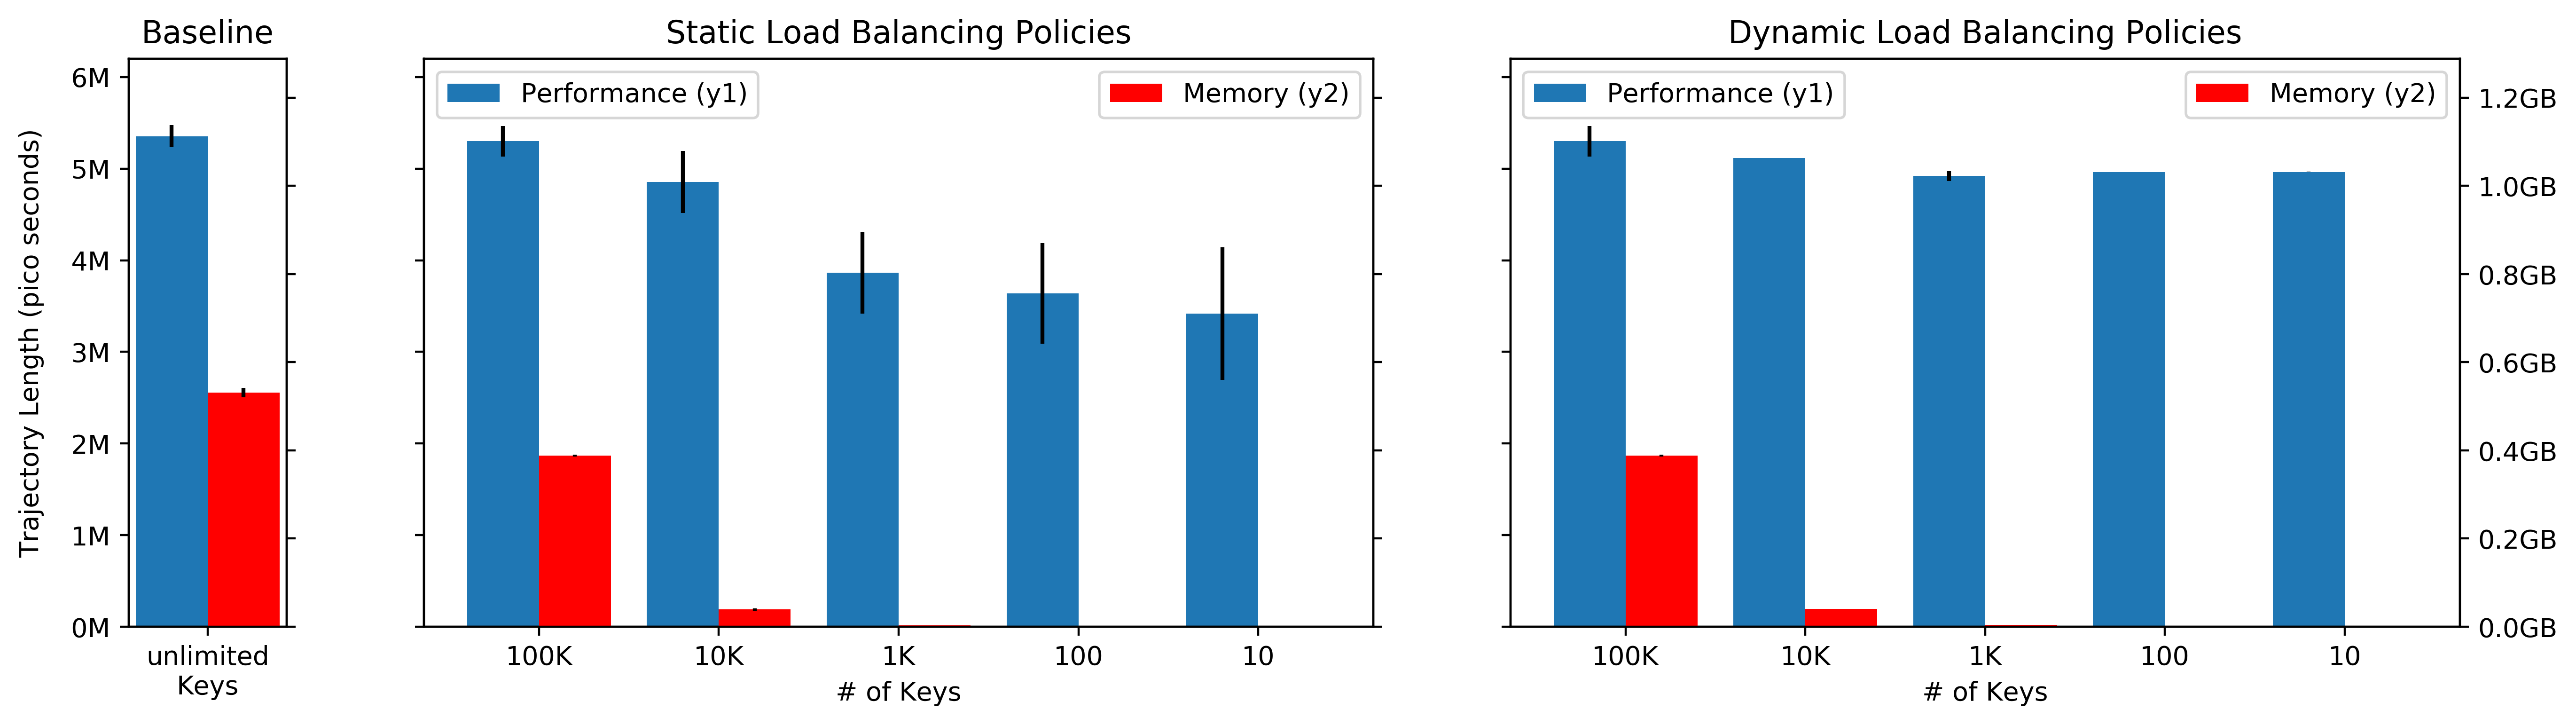
\includegraphics[width=1\textwidth]{figures/methodology-tradeoff.png}\\
  \caption{The optimal cache size must strike a balance between performance and
  resoure utilization. Here we show the trade-off for a static load balancing
  policy that evicts keys when the cache reaches a certain size. For this
  configuration, a 100K key cache has the best performance/utilziation, despite
  the keyspace being 250K keys. \label{fig:methodology-tradeoff}}
\end{figure*}

\subsection{The Need for Dynamic Load Balancing Policies}

% why is the performance lower for smaller caches?
Despite the memory savings, our results suggest that dynamic load balancing
policies could save even more memory.  The left two plots in
Figure~\ref{fig:methodology-tradeoff} show that a 100K key cache is sufficient
as a static policy but the top graph in Figure~\ref{fig:futurework-regimes}
indicates that the value should be much smaller. That graph shows that the
beginning of the run is characterized by many reads to a small set of keys and
the end sees much lower reads per second to a larger keyspace. Specifically, it
shows only about 100 keys are active in the latter half of the run, so a
smaller cache should indeed suffice. 

After analyzing traces, we see that the 100 key cache is insufficient because
LevelDB cannot service the read-write traffic. By limiting the size of the
cache, some reads must traverse up the ParSplice cache hierarchy to the
persistent database.  According to Figure~\ref{fig:futurework-regimes}, the
read requests arrive at 750 reads per second in addition to the writes that
land in each tier (about 300 puts/second, some redundant). This traffic
triggers a LevelDB compaction and reads block and eventually pile up, resulting
in very slow progress. Traces verify this hypothesis and show reads getting
backed up as the read/write ratio explodes. To recap, small caches incurr too
much load on LevelDB at the beginning of the run but smaller caches should
suffice after the initial read flash crowd passes because the keyspace is far
less active, so we need a two part load balancing policy.

% why is it awesome.
%Mantle controls how to distribute or concentrate file system metadata and helps
%users quantify the effects of load balancing.  The paper identified effective
%file system load balancing policies and tested them under metadata-intensive
%workloads. The Greedy Spill balancer, which was based
%on~\cite{patil:fast2011-giga+}, sheds half its load aggressively when there are
%avaiable servers.  The Fill and Spill balancer, which was based
%on~\cite{pai:asplos1998-lard} sheds a fraction of the load only when the server
%is overloaded. Finally, the Adaptable balancer, which was based
%on~\cite{weil:sc2004-dyn-metadata, weil:osdi2006-ceph}, sheds a fraction of the
%load frequently. Mantle is also a powerful debugging tool.

%HXHIM is a good fit because it has migration mechanisms for load balancing
%\begin{itemize} \item bulk operations (\texttt{put/get()}) \item key
%partitioners \item secondary indices \end{itemize} \item we need a way to
%learn these regimes \begin{itemize} \item Figure~\ref{keyspace-regimes-4hr}
%shows the same phases as 100K but that the timestamps affected by delay
%\end{itemize} \end{itemize}
%
% What is Mantle?
% How does it work?
%It was built on CephFS, the file system above Ceph, so it inherits many of
%characteristics of the CephFS architecture, like the dedicated metadata cluster
%and heartbeat mechanisms shown at the top of Figure~\ref{fig:arch-mantle}.
%Each metadata server manages differently sized subtrees of the logical
%namespace and migration decisions are made synchronously, every 10 seconds.
%CephFS already had the mechanisms for load balancing, namely the ability to
%measure the load on a subtree, to migrate subtrees, and to partition subtrees
%into smaller subtrees, but it had hard-coded, ad-hoc policies for guiding the
%migrations.  Mantle reads user-defined policies written in Lua and returns
%decisions for how load should be migrated given the state of the cluster and
%the behavior of the workload. The hooks in Figure~\ref{fig:arch-mantle} show
%where CephFS calls out to the Mantle library to make decisions. While the
%decisions were made by Mantle, CephFS used its internal mechanisms to do the
%load balancing.

% What is the status?
%It was merged\footnote{https://github.com/ceph/ceph/pull/5155} and is starting
%to get users who are frustrated with the hard-coded load balancing policies
%that are shipped with CephFS. It was re-implemented using the ``programmable
%storage" approach~\cite{sevilla:eurosys17} to reduce lines of code for doing
%things like versioning and distributing balancer version.  Although Mantle is
%heavily integrated the daemons that compose an Ceph cluster, using Ceph's
%naming conventions and internal libraries like Ceph's version of protocol
%buffers, there is no reason that it cannot be extracted.
%
%\begin{figure}[tb]
%  \noindent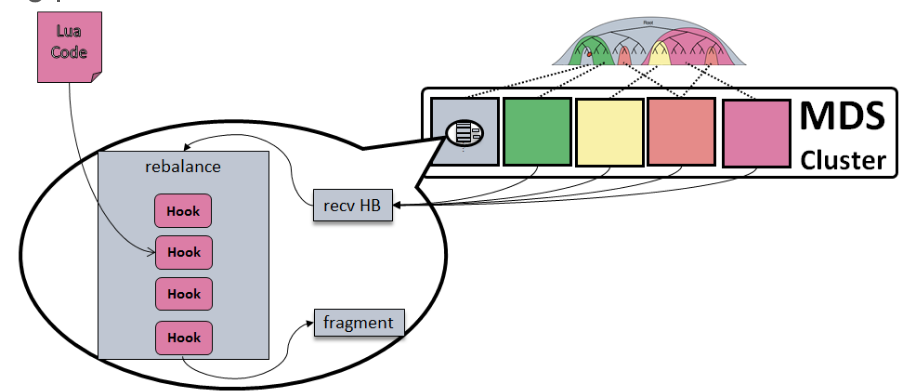
\includegraphics[width=19pc,angle=0]{figures/arch-mantle.png}\\
%  \caption{The Mantle API lets adminstrators control load balancing by
%  changing the poicies for how to distribution or concentrate file system
%  metadata. It was merged into CephFS and inherits many aspects of that
%  architecture. Although it has the load balancing structure and logic from
%  CephFS (gray boxes), the actual API is not dependent on that code base.}
%  \label{fig:arch-mantle}
%\end{figure}
%\begin{figure}[tb]
%  \noindent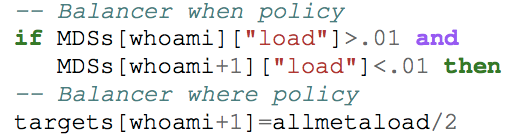
\includegraphics[width=19pc,angle=0]{figures/arch-mantle-example.png}\\
%  \caption{The Greedy Spill balancer written in Lua using the Mantle API.}
%  \label{fig:arch-mantle-example}
%\end{figure}
%

The right most graph of Figure~\ref{fig:methodology-tradeoff} shows the results
of using the Mantle API, described in
Section~\S\ref{sec:mantle-dynamic-load-balancing} to program a dynamic load
balancing policy with two phases into ParSplice:

\begin{itemize}
  \item unlimited growth: cache increases on every put
  \item \(n\) key limit: cache maintained at this size
\end{itemize}

We trigger the policy switch at 100K keys to absorb the flash crowd at the
beginning of the run. Once triggered, keys are evicted to bring the size of the
cache down to the threshold and the least recently keys are actively evicted.
In that figure, the cache sizes are along the \(x\)-axis.

% results: same level of performance can be achived 
The dynamic policies show better performance than the single \(n\) key
policies. The performance and memory utilization for 100K is the same as the
100K bar in the middle graphs but the rest reduce the size of the keyspace
after the read flash crowd. This reduced the read/write traffic on the
persistent database and reduces the amount of stalls.  The worst performing
policy is the 10 key cache, which achieves 94\% of the performance while only
using 40KB of memory. 

% caveats: it is calculating 90% of the trajectory, memory value reported is final
\subsubsection*{Caveats}

The results from the right most graph in Figure~\ref{fig:methodology-tradeoff}
are slightly deceiving for three reason: (1) segments take longer to generate
later in the run, (2) the memory footprint is the value at the end of 2.5
hours, and (3) this policy only works well for the 2.5 hour run.  For (1), the
curving down of the simulation vs. wall-clock time is shown in
Figure~\ref{fig:methodology-trajectory}; as the nanoparticle grows it takes
longer to generate segments so by the time we reach 2.5 hours, over 90\% of the
trajectory is already generated.  For (2), the memory footprint is around 0.4GB
until we reach 100K keys. In Figure~\ref{fig:methodology-tradeoff} we plot the
final value. For (3), Figure~\ref{fig:methodology-trajectory} shows that the
cache fills up with 100K keys at time x and its size is reduced to the size
listed in the legend.  The curves stay close to ``Unlimited" for up to an hour
after the cache is reduced but eventually flatten out as the persistent
database gets overloaded. 10K and 100K follow the ``Unlimited" curve the
longest and are sufficient policies for the 2.5 hour runs but anything longer
would need a different dynamic load balancing policy.

\begin{figure}[tbh]
  \noindent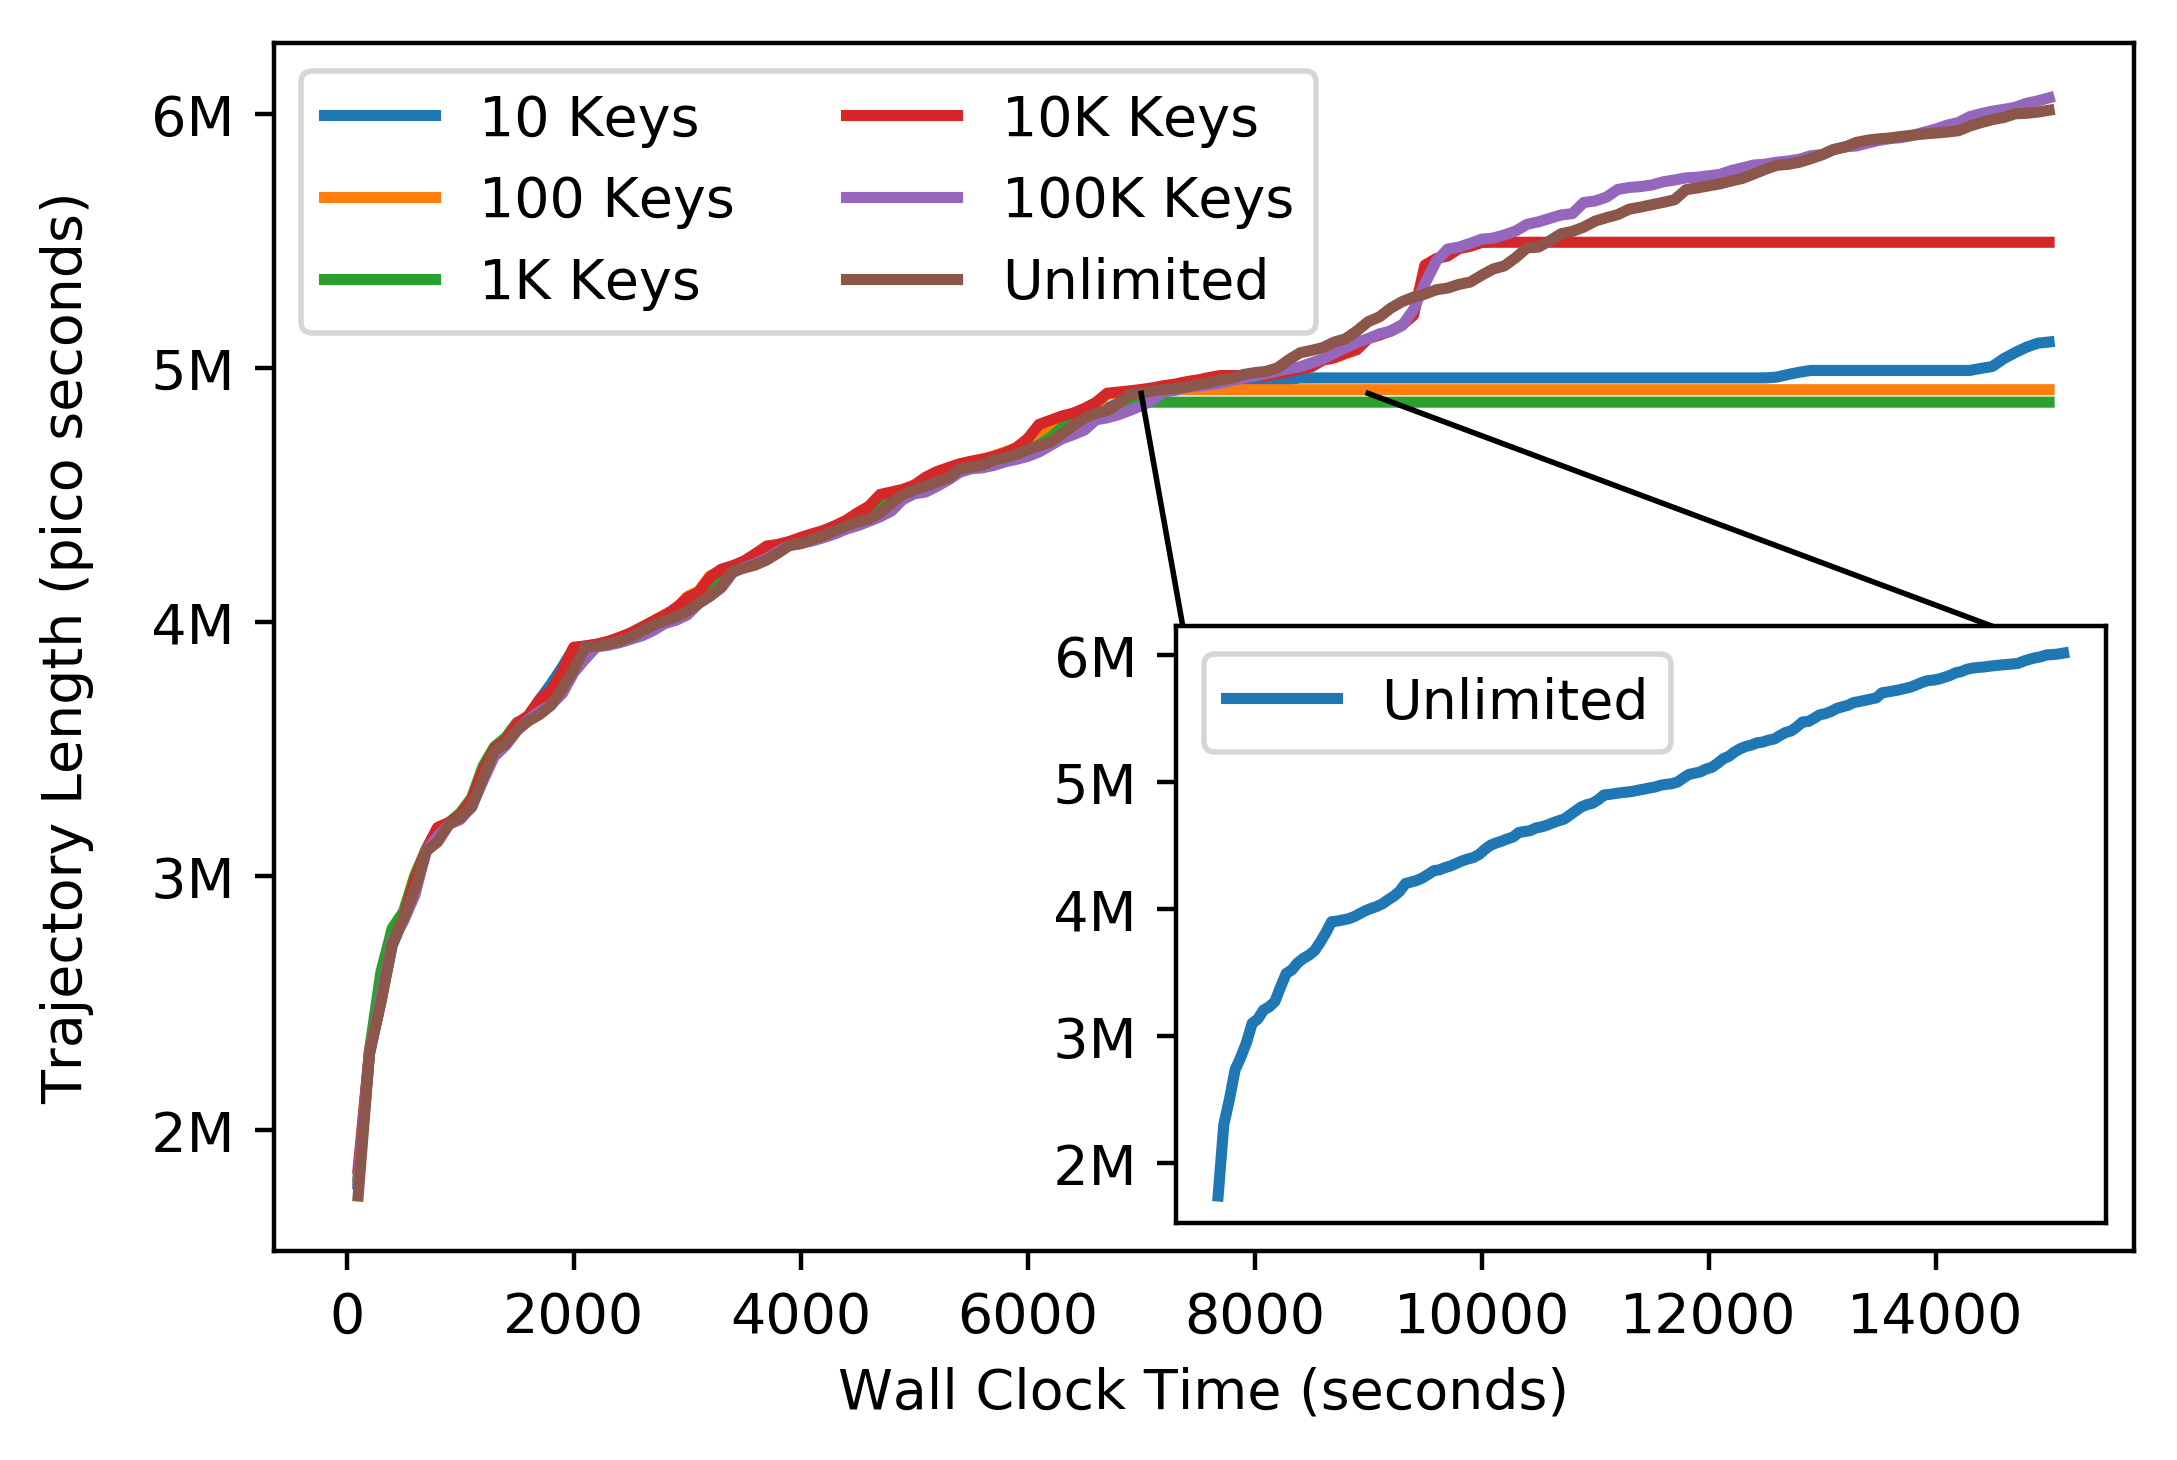
\includegraphics[width=0.45\textwidth]{figures/methodology-trajectory.png}\\
  \caption{The optimal cache size must strike a balance between performance and
  the keyspace being 250K keys. \label{fig:methodology-trajectory}}
\end{figure}

% wht the result is still valie
Despite these caveats, the result is still valid: we found a dynamic load
balancing policy that absorbs the cost of a high read throughput on a small
keyspace and reduces the memory pressure for a 2.5 hour run. The problem is
that the thresholds in these policies does not work for different setups ({\it
i.e.} different ParSplice parameters, number of worker nodes, and job lengths).
We need a way to identify what thresholds we should use for different job
permutations.

\subsection{Machine Learning Keyspace Activity}
%\begin{itemize}
%  \item C bindings for Mantle
%\end{itemize}
%
%\subsection{Pluggable Interfaces}
%
%\begin{figure}[tb]
%  \noindent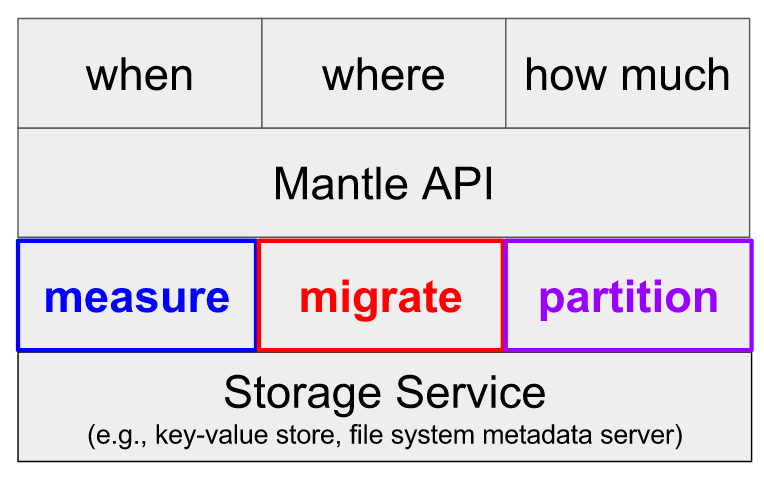
\includegraphics[width=19pc,angle=0]{figures/mantle-pluggable-interfaces.png}\\
%  \caption{The storage service must: \textcolor{blue}{\textbf{measure}}
%  resource usage, \textcolor{red}{\textbf{migrate}} resources, and
%  \textcolor{purple}{\textbf{partition}} resources. }
%  \label{fig:mantle-pluggable-interfaces}
%\end{figure}
%
%\subsubsection{Measure}
%
%The metrics measured should help the system decide ``when" to migrate server
%load. They should:
%
%\begin{itemize}
%  \item tell us about the state of the server or cluster
%  \item provide some value of load, so we can partition/send it
%\end{itemize}
%
%In Ceph: global and local metrics ({\it e.g.}, CPU utilization, file system operation counts) \\
%
%In HXHIM: ???\\
%
%\subsubsection{Migrate}
%
%In Ceph: \texttt{export\_dir()}
%
%In HXHIM: \texttt{mdhimBPut()}, \texttt{mdhimBGet()}, ``adjusting ... keys" ???
%
%\subsubsection{Partition}
%
%In Ceph: subtrees and directory fragments
%
%In HXHIM: secondary indices, cursor types, bul operations

\section{Conclusion}

\begin{enumerate}
  \item analysis of Parsplice keyspace
  \item using a modern distributed kv store
  \item positive effects of Mantle
\end{enumerate}


\bibliographystyle{ACM-Reference-Format}
\bibliography{references} 

\end{document}
